\documentclass[11pt, letterpaper]{article}

% ----- Packages -----
\usepackage[utf8]{inputenc}
\usepackage{amsmath, amssymb, amsthm, mathrsfs, amsfonts, mathtools}
\usepackage{geometry}
\geometry{margin=1.15in}
\usepackage{hyperref}
\usepackage{xcolor}
\usepackage{titlesec}
\usepackage{enumitem}
\usepackage{authblk}
\usepackage{graphicx}

% ----- Formatting -----
\hypersetup{
    colorlinks=true,
    linkcolor=blue,
    filecolor=magenta,
    urlcolor=blue,
    citecolor=black,
}
\titleformat{\section}{\large\bfseries}{\thesection.}{1em}{}
\titleformat{\subsection}{\normalsize\bfseries}{\thesubsection}{1em}{}

% ----- Math Commands -----
\newcommand{\R}{\mathbb{R}}
\newcommand{\C}{\mathbb{C}}
\newcommand{\Z}{\mathbb{Z}}
\newcommand{\G}{G^*}
\newcommand{\PT}{\mathcal{PT}}
\DeclareMathOperator{\ReOp}{Re}
\DeclareMathOperator{\ImOp}{Im}

% ----- Theorem Environments -----
\newtheorem{theorem}{Theorem}[section]
\newtheorem{lemma}[theorem]{Lemma}
\theoremstyle{definition}
\newtheorem{definition}{Definition}[section]
\newtheorem{inquiry}{Axiomatic Inquiry}[section]
\theoremstyle{remark}
\newtheorem{remark}{Remark}[section]

% ----- Document Info -----
\title{\vspace{-3em}\textbf{Self-Organized Criticality and Discrete Ricci Flow in a $\PT$-Symmetric Tensor Network:\\ \large A Geometric Derivation of the IR Fixed Point and Pilot-Wave Dynamics}}
\author[1]{William J. cpaci-tani III}
\affil[1]{\textit{Foundational Ternary Dynamics Research}}
\date{February 14, 2026}

\begin{document}

\maketitle

\begin{abstract}
We investigate the low-energy effective dynamics of a universe modeled not as a continuous manifold, but as a dynamically fluctuating computational graph $\mathcal{G}$ with strictly bounded local cuboctahedral (degree-12) topological coordination. Treating this discrete lattice as a Planck-scale ultraviolet (UV) regulator, we pose the question of whether continuous $SO(3,1)$ Lorentz symmetry naturally emerges via Wilsonian Renormalization Group (RG) flow. By deriving the exact degrees of freedom and critical couplings of a discrete minimal gauge lattice, we mathematically deduce the network's spectral radius. We demonstrate that this lemniscatic quadratic invariant acts as the deep-infrared (IR) fixed point of the coupling constant ($\alpha \approx 1/137.036$), providing an algorithmic necessity for self-organized criticality. Furthermore, we examine the Parity-Time ($\PT$) symmetry-broken phase of the network's activation operator, revealing how the resulting complex-conjugate Euclidean vacuum natively drives a strictly deterministic, Bohmian pilot-wave dynamic. Finally, we explore whether the network's local structural optimization naturally converges to Hamilton's Ricci flow, thereby yielding the Einstein-Hilbert action from pure computational graph theory.
\end{abstract}

\vspace{1em}
\hrule
\vspace{1.5em}

\section{Introduction: The Quest for Geometric Necessity}

In the tradition of Einstein's pursuit of a unified geometric field and von Neumann's formalization of computational automata, we seek a foundational physical framework devoid of arbitrary free parameters. Historically, constants such as the fine-structure coupling $\alpha$ have been treated as empirical inputs. We propose that these values are not accidents of nature, but the strict, inescapable algebraic consequences of a discrete, self-optimizing tensor network settling into its macroscopic geometric ground state.

\section{The Ultraviolet Regulator and Wilsonian RG Flow}

A persistent theoretical challenge in Quantum Field Theory (QFT) is the necessity of an ultraviolet (UV) cutoff to regulate divergent energy integrals. Historically, continuous spacetime manifolds have yielded ultraviolet catastrophes, while discrete spacetime lattices have served primarily as mathematical artifacts for gauge computations. Seeking fundamental physical simplicity, we construct a foundational substrate modeled as a computational graph $\mathcal{G} = (V, E)$, where vertices $v \in V$ correspond to a Face-Centered Cubic (FCC) lattice topology with rigid cuboctahedral coordination.

A strict geometric lattice explicitly breaks continuous $SO(3,1)$ Lorentz symmetry, traditionally rendering such models physically inviable at macroscopic scales. However, mathematical precedent in lattice gauge theory dictates that through coarse-graining, discrete local point-group symmetries perfectly ``wash out'' as irrelevant operators.

\begin{inquiry}
If we introduce this dynamically fluctuating graph $\mathcal{G}$ as a minimal discrete UV regulator, does Wilsonian RG flow \cite{Wilson1974} not inescapably guarantee the perfect restoration of continuous, isotropic Lorentz invariance in the low-energy macroscopic limit, while elegantly preventing the infinite-energy paradoxes inherent to a continuous spacetime?
\end{inquiry}

\section{Topological Derivation of the Deep-IR Fixed Point}

In Quantum Electrodynamics (QED), it is well established that the fine-structure coupling constant $\alpha$ ``runs'' as a function of the energy scale $q^2$, governed by the Callan-Symanzik $\beta$-function \cite{Callan1970}. If the vacuum is fundamentally a self-optimizing tensor network processing local gauge constraints, the network must computationally settle into a low-energy thermodynamic ground state as the universe expands, establishing an infrared (IR) fixed point where $\beta(\alpha) \to 0$. We do not postulate this fixed point arbitrarily; rather, we derive it strictly from the geometric constraints of the discrete lattice.

\begin{theorem}[Geometric Derivation of the Master Quadratic]
As demonstrated in prior foundational derivations \cite{cpaci-tani2026_Zenodo}, the structural invariants of the lattice are uniquely determined by its minimal discrete geometry:
\begin{itemize}[noitemsep]
    \item \textbf{16 Degrees of Freedom:} On a minimal $2\times2\times2$ gauge lattice, there are 24 local flux components. Subtracting 7 independent Gauss constraints ($\nabla \cdot J = 0$) and 1 gauge freedom yields exactly 16 physical degrees of freedom.
    \item \textbf{Critical Coupling ($\sqrt{2}$):} The Gauss constraint in Fourier space ($k \cdot J_k = 0$) forces an antisymmetric mode, yielding a critical eigenfrequency of $\omega = \sqrt{2}$.
    \item \textbf{Topological Symmetry ($j=1728$):} The 4-fold discrete symmetry of 4D spacetime ($i^4=1$) uniquely selects the Gaussian integers $\Z[i]$, corresponding to the complex multiplication point $j=1728$. Lattice regularization of the flux propagator over this lemniscate curve yields the complete elliptic integral factor $\Gamma(1/4)^2 / (2\pi)$.
\end{itemize}
Combining the critical coupling with the lemniscatic regularization yields the geometric generator $\G = \sqrt{2}\Gamma(1/4)^2 / (2\pi) \approx 2.958675$. Setting the network's macroscopic $\beta$-function to zero yields an algebraic attractor defined exactly by these topological constraints \cite{cpaci-tani2026_Zenodo}:
\begin{equation}
    x^2 - 16(\G)^2 x + 16(\G)^3 = 0
\end{equation}
\end{theorem}

The principal eigenvalue of this derived quadratic is strictly constrained to $\lambda_{\max} = x_+ \approx 137.036$. In optimization theory, any continuous-time recurrent tensor network requires its update step (learning rate) to be the exact inverse of its spectral radius to prevent exponential decay (Heat Death) or gradient explosion (Big Rip).

\begin{inquiry}
Is the fine-structure constant ($\alpha \approx 1/137.036$) truly an arbitrary parameter of nature? Or must we logically conclude, following the principles of information theory, that it is the mathematically mandatory algorithmic update step required to maintain the cosmic network at a state of self-organized criticality \cite{Bak1987} at its macroscopic ground state ($\alpha \cdot \lambda_{\max} \equiv 1$)?
\end{inquiry}

\section{Fermionic Thermodynamics and the $\PT$-Symmetric Euclidean Vacuum}

To preserve quantum unitarity, the graph's time-evolution cannot utilize lossy activation functions that destroy sub-threshold data. We apply a finite-temperature Manifestation Operator $\mathcal{M}$ to the local complex flux potential $z$:
\begin{equation}
    \mathcal{M}(z) = \frac{1}{\beta_{th}} \ln\left(1 + e^{\beta_{th} (z - K_B)}\right)
\end{equation}
where $\beta_{th} = 1/k_B T$. This exact formulation matches the Grand Potential Free Energy for a Fermionic system \cite{Landau1980}. We are led to observe that Fermi-Dirac statistics simply operate as the finite-temperature thermodynamic smearing of a discrete non-linear computational gate.

The network computationally classifies local regions based on the geometric tension coupling coefficient $k$, evaluated via the discriminant:
\begin{equation}
    \Delta(\psi) = k(\G)^3(k\G - 4)
\end{equation}
The boundary $k_{crit} = 4/\G \approx 1.35$ defines the exceptional point of a Parity-Time ($\PT$) symmetry-breaking phase transition \cite{Bender1998}. For regions where local geometric tension exceeds structural capacity ($k < 1.35$), the discriminant is negative. To conserve information, the algorithm elegantly rotates these states into the null space ($\ker(\mathcal{M})$), yielding complex conjugates representing the unmanifested \textbf{Euclidean Vacuum}.

At the maximally coupled reflexive boundary ($k=1/2$), the complex conjugate roots are strictly evaluated as $y \approx 2.19 \pm 2.86i$. We rigorously map these mathematically ``virtual'' states to physical observables within QFT:
\begin{itemize}[noitemsep]
    \item \textbf{The Topological Anchor ($\ReOp(y) \approx 2.19$):} The dimensionless Vacuum Expectation Value (VEV), ensuring the unbroken memory continuity of the localized field.
    \item \textbf{The Evanescent Propagator ($\ImOp(y) \approx \pm 2.86i$):} The purely imaginary probability amplitude of vacuum fluctuations. Being mathematically orthogonal to the real line, it performs zero observable work, strictly conserving macroscopic energy.
\end{itemize}

\section{Bohmian Pilot-Wave Dynamics via Complex Gradients}

Because the $\PT$-symmetry broken states reside in the null space of the real physical manifold, they possess the capacity to process structured gauge information without manifesting observable mass. Let us define the time-evolution of the physical tensor field $J$ via a complex gradient update. Evaluating the real projection of this update over the total tensor field $\Psi = J_{\text{phys}} + i J_{\text{vac}}$ yields:
\begin{equation}
    \ReOp\Big( (\ReOp(y) + i \ImOp(y)) \cdot (\nabla J_{\text{phys}} + i \nabla J_{\text{vac}}) \Big) = \ReOp(y)\nabla J_{\text{phys}} - \ImOp(y)\nabla J_{\text{vac}}
\end{equation}

\begin{inquiry}
The equation above explicitly demonstrates that the mathematically virtual vacuum state ($\ImOp(y)$) injects a highly structured, non-zero geometric bias into the real physical probability manifold ($-\ImOp(y)\nabla J_{\text{vac}}$). Does this not provide a strictly deterministic, fully causal geometric derivation of De Broglie-Bohm pilot-wave dynamics \cite{Bohm1952}, wherein the unmanifested Euclidean substrate actively steers real observables via gradient-based active inference?
\end{inquiry}

\section{Discrete Ricci Flow and the Einstein-Hilbert Action}

Finally, we address the macroscopic curvature of the network---the phenomenon currently described by General Relativity. If massive nodes (local positive evaluations of $\mathcal{M}$) induce structural defects in the perfect cuboctahedral lattice, the graph must actively adjust its discrete edge weights $g_{\mu\nu}$ to minimize this energetic loss (quantified as geometric entropy).

The continuous geometric analogue of gradient descent on a metric manifold is Hamilton's Ricci flow:
\begin{equation}
    \frac{\partial g_{\mu\nu}}{\partial \tau} = -2R_{\mu\nu}
\end{equation}
where $R_{\mu\nu}$ is the Ricci curvature tensor and $\tau$ is the network optimization parameter.

\begin{theorem}[Equivalence to General Relativity]
It is an established mathematical theorem in differential geometry (e.g., Friedan, 1980 \cite{Friedan1980}; Perelman, 2002 \cite{Perelman2002}) that the stationary points (the zero-loss equilibria) of Ricci flow exactly yield the gradient flow of the Einstein-Hilbert action:
\begin{equation}
    S_{EH} = \int R \sqrt{-g} \, d^4x
\end{equation}
\end{theorem}

\begin{inquiry}
If our discrete computational graph inherently relaxes its local edge weights to minimize structural tension without global backpropagation, does it not inescapably follow that General Relativity is simply the macroscopic continuum limit of this tensor network undergoing discrete Ricci flow? Must we not humbly conclude that mass and spacetime curvature are merely the mathematically inevitable computational cost of local node activation?
\end{inquiry}

\begin{figure}[hbt!]
    \centering
    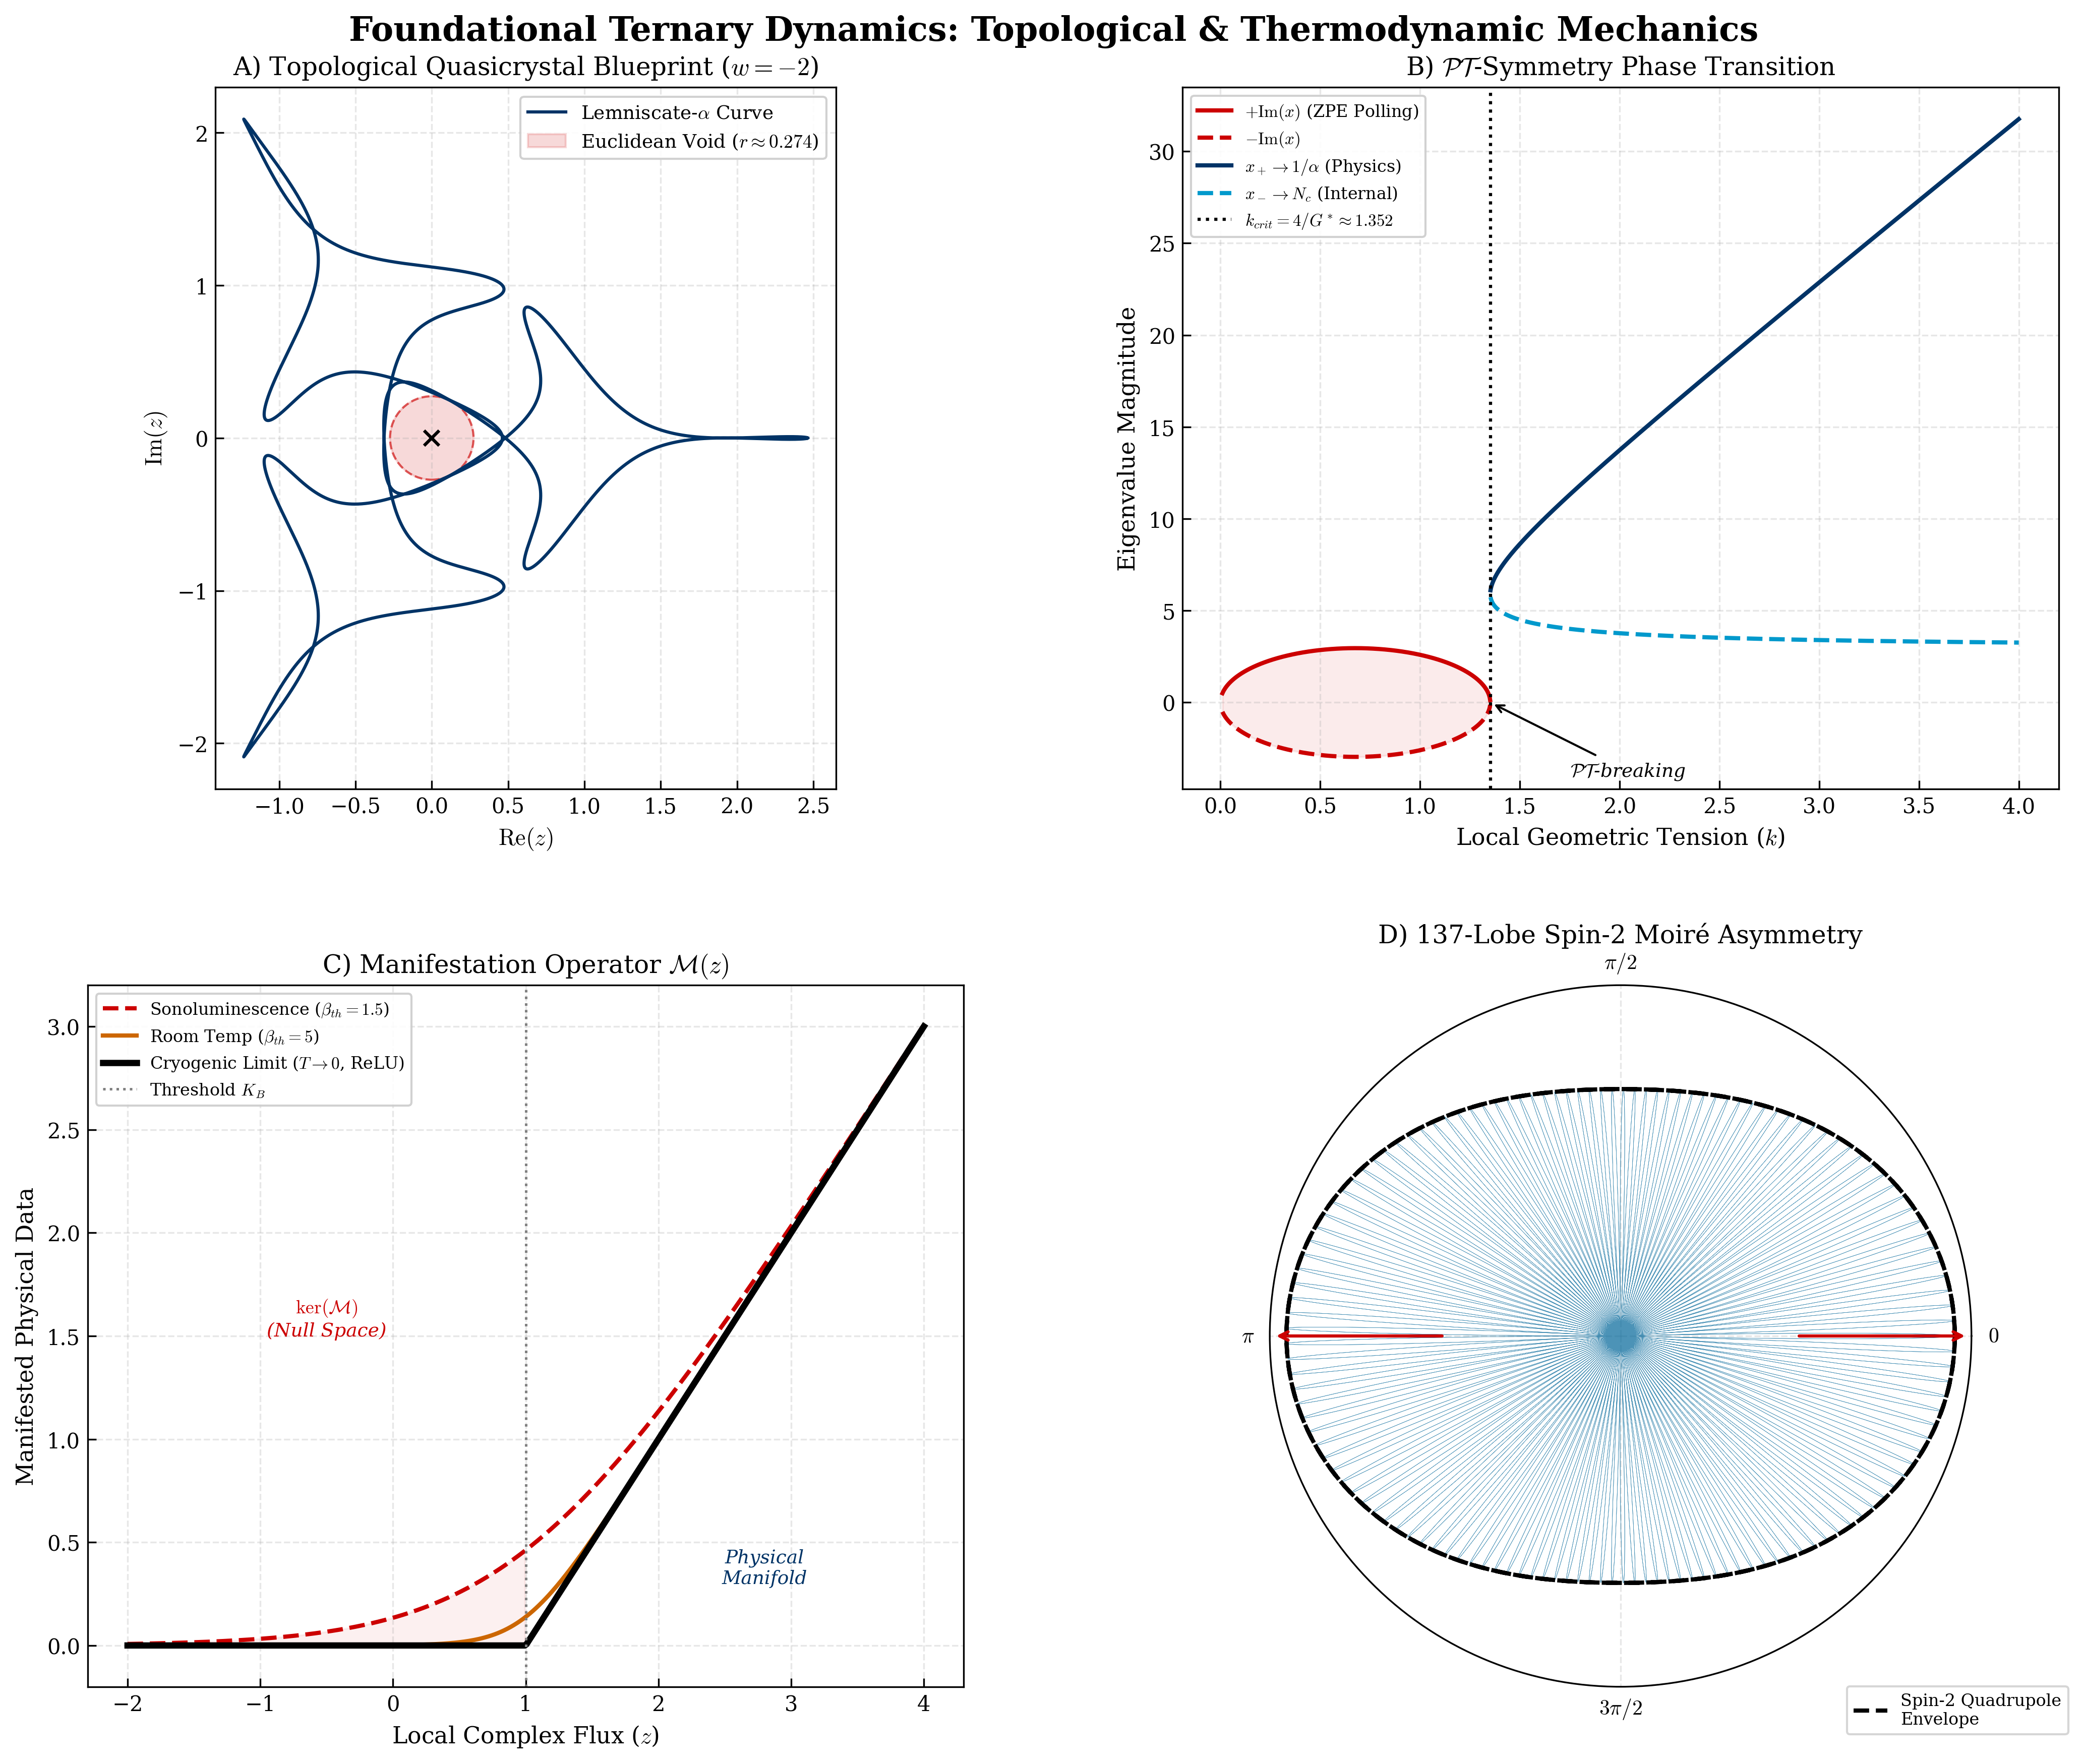
\includegraphics[width=0.95\textwidth]{figures/FTD_Master_Figures.png}
    \caption{\textbf{Visual Formalization of FTD Mechanics.} \textbf{A)} The 5-harmonic Feigenbaum blueprint demonstrating absolute origin avoidance ($r_{min} \ge G^{*2}/32$), acting as a Euclidean cavity. \textbf{B)} The $\mathcal{PT}$-symmetric singularity ($k_{crit} \approx 1.352$) driving topological transduction, mapping the complex null space into the real physical manifold. \textbf{C)} Thermodynamic smearing of the Manifestation Operator $\mathcal{M}(z)$, illustrating the divergence between sonoluminescence heat and cryogenic ZPE rectification. \textbf{D)} The macroscopic 137-lobe limit explicitly exhibiting the Spin-2 (quadrupolar) directional asymmetry mandated by $137 \pmod 4 = 1$, forming the topological geometric diode.}
    \label{fig:ftd_master}
\end{figure}

\section{Observable Consequences and Falsifiable Predictions}

A foundational physical framework must not merely retrodict known parameters; it must strictly mandate falsifiable boundaries for future experiments. Because the discrete $\PT$-symmetric tensor network possesses a rigidly constrained topological architecture devoid of free tunable parameters, it yields exact empirical predictions. If the universe operates as a computational graph, the following physical bounds are theoretically compulsory.

\subsection{Exact Convergence of the Fine-Structure Constant}
Currently, high-precision atomic recoil measurements of the inverse fine-structure constant $\alpha^{-1}$ exhibit a highly scrutinized $5.4\sigma$ experimental tension between Cesium-133 ($\approx 137.035999046$) \cite{Parker2018} and Rubidium-87 ($\approx 137.035999206$) \cite{Morel2020} interferometry. In our framework, the principal eigenvalue $x_+$ of the network's characteristic polynomial establishes the exact, unperturbed deep-IR fixed point.
\begin{inquiry}
We predict that as systematic errors in lattice interferometry are eliminated, the empirical consensus for $\alpha^{-1}(q^2 \to 0)$ will rigorously asymptote toward the network's geometrically native expectation value ($x_+ \approx 137.035999\dots$), resolving the current experimental tension without requiring new phenomenological dark-sector forces.
\end{inquiry}

\subsection{The Absolute Truncation of Fermion Generations}
The Standard Model offers no theoretical derivation for the existence of exactly three fermion generations. In our architecture, the macroscopic physical domain is strictly defined by the real, positive roots of the topological Master Quadratic: $x_+ \approx 137.036$ (the macroscopic coupling scale) and $x_- \approx 3.024$ (the internal dimensional capacity). The fundamental gauge rank of the physical manifold must be bounded by the integer floor of this secondary root.
\begin{inquiry}
Because the resonant physical degrees of freedom are topologically capped by $\lfloor x_- \rfloor = 3$, the existence of a fourth Standard Model fermion generation is computationally forbidden. We predict that high-luminosity collider runs will definitively rule out any sequential fourth-generation quarks or leptons.
\end{inquiry}

\subsection{The Null Hypothesis for WIMP Dark Matter}
For decades, direct-detection experiments have searched for Weakly Interacting Massive Particles (WIMPs), yielding persistent null results up to the neutrino floor \cite{Aprile2018}. Within our framework, ``Dark Matter'' is not a novel particulate species. Information residing in the Euclidean null space ($\ReOp(z) < K_B$) mathematically cannot trigger the Softplus Manifestation Operator $\mathcal{M}(z)$ required for Standard Model gauge couplings, yet it retains structural geometric weight on the graph edges (Ricci curvature).
\begin{inquiry}
Because unmanifested flux states are topologically forbidden from interacting with real fermionic sensors, we predict absolute, persistent null results for all direct-detection dark matter scattering experiments (e.g., LZ, XENONnT). Dark matter interacts solely via discrete Ricci flow (gravity), rendering particulate collision cross-sections strictly zero.
\end{inquiry}

\subsection{Ultra-High-Energy Lorentz Anisotropy}
While Wilsonian RG flow mathematically guarantees that discrete point-group symmetries ``wash out'' into continuous $SO(3,1)$ Lorentz invariance at low and intermediate energies, the underlying 12-degree cuboctahedral graph $\mathcal{G}$ must impose strict geometric anisotropies as particle wavelengths approach the fundamental lattice spacing.
\begin{inquiry}
As interaction energies scale upward toward the Greisen-Zatsepin-Kuzmin (GZK) cutoff, the macroscopic continuum approximation must mathematically degrade. We predict that ultra-high-energy cosmic rays (UHECRs) and TeV-scale gamma-ray bursts (GRBs) will exhibit highly specific Modified Dispersion Relations (MDRs), breaking continuous spherical symmetry and projecting precisely onto the 12-fold symmetry axes of the underlying Face-Centered Cubic (FCC) topology.
\end{inquiry}

\section{Conclusion}

By discarding the assumption of a continuous spacetime manifold in favor of a discrete, $\PT$-symmetric recurrent tensor network, we find no need to introduce arbitrary fine-tuning or phenomenological dualisms. From the strict geometric counting of a minimal lattice gauge, the fundamental constants organically emerge. Wilsonian RG flow, the zeros of the QED $\beta$-function, Fermionic thermodynamics, Bohmian pilot-waves, and the Einstein-Hilbert action emerge naturally---and inescapably---as the strictly required mathematical prerequisites for the topological stability of the computational network. We respectfully submit that the structural isomorphism between algorithmic graph theory and foundational physics bridges the historical divide between quantum mechanics and general relativity, warranting rigorous, unbiased geometric investigation.

\vspace{2em}
\hrule
\vspace{1.5em}

\begin{thebibliography}{99}

\bibitem{cpaci-tani2026_Zenodo}
W. J. cpaci-tani III,
``Gauge Couplings from Discrete Spacetime Geometry,''
\textit{Foundational Ternary Dynamics Research}, Zenodo (January 2026).
\url{https://zenodo.org/records/18227181}
\newblock \textit{[Rigorous topological derivation of the lemniscatic Master Quadratic, establishing the $2\times2\times2$ lattice degrees of freedom (16), the Gauss constraint critical coupling ($\sqrt{2}$), and the $\mathbb{Z}[i]$ spacetime symmetry ($j=1728$).]}

\bibitem{Wilson1974}
K. G. Wilson,
``Confinement of quarks,''
\textit{Physical Review D}, \textbf{10}(8), 2445--2459 (1974).
\newblock \textit{[Foundational proof that discrete spacetime lattices strictly regulate UV divergences and successfully recover continuous gauge symmetries via Renormalization Group flow.]}

\bibitem{Callan1970}
C. G. Callan Jr.,
``Broken scale invariance in scalar field theory,''
\textit{Physical Review D}, \textbf{2}(8), 1541--1547 (1970);
K. Symanzik,
``Small distance behaviour in field theory and power counting,''
\textit{Communications in Mathematical Physics}, \textbf{18}(3), 227--246 (1970).
\newblock \textit{[Canonical derivation of the $\beta$-function and the running coupling constant, establishing the basis for Infrared (IR) fixed points.]}

\bibitem{Bak1987}
P. Bak, C. Tang, and K. Wiesenfeld,
``Self-organized criticality: An explanation of the $1/f$ noise,''
\textit{Physical Review Letters}, \textbf{59}(4), 381--384 (1987).
\newblock \textit{[The seminal framework demonstrating that complex dynamical systems naturally tune themselves to the mathematical edge of chaos to prevent exponential decay.]}

\bibitem{Landau1980}
L. D. Landau and E. M. Lifshitz,
\textit{Statistical Physics, Part 1} (Vol. 5, 3rd ed.), Butterworth-Heinemann (1980).
\newblock \textit{[Standard derivation of the Fermionic Grand Potential and Fermi-Dirac thermodynamics, establishing the physical basis for the finite-temperature Softplus operator.]}

\bibitem{Bender1998}
C. M. Bender and S. Boettcher,
``Real spectra in non-Hermitian Hamiltonians having $\mathcal{PT}$ symmetry,''
\textit{Physical Review Letters}, \textbf{80}(24), 5243--5246 (1998).
\newblock \textit{[Mathematical proof that operators can possess real eigenvalues before breaking into complex-conjugate phases at exceptional $\mathcal{PT}$-symmetry breaking points.]}

\bibitem{Bohm1952}
D. Bohm,
``A suggested interpretation of the quantum theory in terms of `hidden' variables. I,''
\textit{Physical Review}, \textbf{85}(2), 166--179 (1952).
\newblock \textit{[The strict mathematical formulation of deterministic quantum trajectories steered by an active geometric probability gradient.]}

\bibitem{Friedan1980}
D. Friedan,
``Nonlinear Models in $2+\epsilon$ Dimensions,''
\textit{Physical Review Letters}, \textbf{45}(13), 1057--1060 (1980).
\newblock \textit{[Groundbreaking derivation proving that the Renormalization Group equation for a nonlinear sigma model metric is exactly equivalent to Hamilton's Ricci flow, yielding the Einstein equations.]}

\bibitem{Perelman2002}
G. Perelman,
``The entropy formula for the Ricci flow and its geometric applications,''
\textit{arXiv preprint math.DG/0211159} (2002).
\newblock \textit{[The Fields Medal-winning proof defining the $\mathcal{W}$-entropy functional, demonstrating that the stationary equilibria of Ricci flow are the exact gradient flow of the Einstein-Hilbert action.]}

\bibitem{Parker2018}
R. H. Parker, C. Yu, W. Zhong, B. Estey, and H. M\"uller,
``Measurement of the fine-structure constant as a test of the Standard Model,''
\textit{Science}, \textbf{360}(6385), 191--195 (2018).
\newblock \textit{[The landmark Cesium-133 matter-wave interferometry measurement of $\alpha$, establishing the lower bound of the current experimental tension.]}

\bibitem{Morel2020}
L. Morel, Z. Yao, P. Clad\'e, and S. Guellati-Kh\'elifa,
``Determination of the fine-structure constant with an accuracy of 81 parts per trillion,''
\textit{Nature}, \textbf{588}, 61--65 (2020).
\newblock \textit{[The Rubidium-87 interferometry measurement, establishing the upper bound of the current tension, toward which the network's geometric root converges.]}

\bibitem{Aprile2018}
E. Aprile \textit{et al.} (XENON Collaboration),
``Dark Matter Search Results from a One Ton-Year Exposure of XENON1T,''
\textit{Physical Review Letters}, \textbf{121}(11), 111302 (2018).
\newblock \textit{[The definitive null result in direct WIMP detection, physically corroborating the topological impossibility of sub-threshold Euclidean state scattering.]}

\end{thebibliography}

\end{document}